\documentclass[conference]{IEEEtran}
\IEEEoverridecommandlockouts
% The preceding line is only needed to identify funding in the first footnote. If that is unneeded, please comment it out.
\usepackage{cite}
\usepackage{graphicx}
\usepackage{array}


%Import the natbib package and sets a bibliography  and citation styles
%\usepackage{natbib}
\usepackage[square,numbers]{natbib}
\usepackage{url}
\bibliographystyle{abbrvnat}
%\setcitestyle{authoryear,open={(},close={)}}


\graphicspath{ {./images/} }
\def\BibTeX{{\rm B\kern-.05em{\sc i\kern-.025em b}\kern-.08em
    T\kern-.1667em\lower.7ex\hbox{E}\kern-.125emX}}
\begin{document}

\title{Sentiment Analysis Report\\
}

\author{
	\IEEEauthorblockN{Daniyar Kultayev}
	\IEEEauthorblockA{\textit{dept. of Computer Science} \\
	\textit{Nazarbayev Univercity}\\
		Astana, Kazkahstan \\
		email Daniyar.Kultayev@nu.edu.kz}
	\and
	\IEEEauthorblockN{Kamalkhan Artykbayev }
	\IEEEauthorblockA{\textit{dept. of Computer Science} \\
	\textit{Nazarbayev Univercity}\\
		Astana, Kazkahstan \\
		email Artykbayev.Kamalkhan@nu.edu.kz}
}

\maketitle

\newcommand{\RT}{Rotten Tomatoes }
\newcommand{\TW}{Sentiment140 }

\begin{abstract}
Artificial Neural Networks are gaining increasing popularity, and are applied in variety of different fields. Particularly, in the area of Natural Language Processing, neural networks have replaced previously used rule based approaches. Moreover, current neural networks are capable of producing impressive results. Namely, different variations of CNNs and LSTMs are having great success in area of Natural Language Processing, Sentiment Analysis. While the field of NLP have moved on to more challenging problems, such as, Aspect Level Sentiment Analysis, the quality of available Datasets also increased. Thus, it raises the question, whether success of current technique is based solely on the methods themselves, or Dataset has its own influence towards the final result.
\end{abstract}

\begin{IEEEkeywords}
Machine Learning, Natural Language Processing, Natural Language Understanding, RNN, LSTM, CNN
\end{IEEEkeywords}

\section{Introduction}

Artificial Neural Networks have played key role in solving number of important problems in the past, and still are widely used in variety of different fields. Particularly, in the area of Natural Language Processing(NLP), recent successes allowed us to have efficient Speech Recognition, Language Translation, or even Sentiment Analysis. Although, we are very far from Natural Language Understanding, still, Sentiment Analysis is considered as a key insight towards achieving it. Thus, most of the current works related to Natural Language Understanding are focused on Sentiment Analysis.

Moreover, recent advancements in Sentiment Analysis using neural networks surpassed previously used Rule Based Grammar Analysis. For instance, neural network based approaches are far superior in terms of speed and accuracy, while they are capable of constructing Syntax Structure of a given sentence. Besides, neural network based approaches are much more flexible, and require significantly less human intervention. Not only that, but also, some of the neural network approaches are unsupervised in terms of training. That is to suggest that, they only need training data to be able to produce results.

Additionally, current advancements in neural networks provided means of analyzing sentences with even better precision. Not only they are capable of accurately determine the sentiment of a given sentence, they are also capable of Aspect Level Sentiment Analysis. 

Aspect Level Sentiment Analysis as grown its popularity in past years, due to the thoroughness of the approach. That is, determining Aspects or Targets of the sentence and evaluating their sentiment based on a given context. In contrast with Sentiment Analysis of the sentence, Aspect Level Sentiment Analysis provides much more deeper evaluation of a sentence. Also, Aspect Level Sentiment Analysis methods, resemble human approach of evaluating sentiment of the sentence.

Besides, most of currently used neural networks adopt the fact that they have to be flexible. Moreover, due to significant differences in language variations, they reject the notion of incorporating statically defined rules. Thus, training process have to be data-driven and unsupervised/semi-supervised.

Therefore, two of the most common neural networks that fit the purpose considered to be: CNN and different variations of RNNs.

\section{Related Work}
While Sentiment Analysis dates back to 2002 \cite{pang-etal-2002-thumbs}, we are still far from Natural Language Understanding.
Moreover, sentiment classification seemed inadequate in cases were structure contained polar sentiments. Thus, it lead to proposition of Aspect Sentiment Classification \cite{Sentiment:Aspect:Hu:2004} as an alternative. Though, admittedly, ASC is much more sophisticated and resource demanding. Nevertheless, with social media influence growth, commercial interest for opinion mining, and sentiment analysis has increased dramatically. Thus, making Sentiment Analysis and ASC as hottest topics in NLP currently.

Therefore, there have been number of attempts towards both Sentiment Analysis and ASC. While RNNs\cite{Hochreiter:1997:LSM:1246443.1246450} date back to 1997, ASC and Sentiment Analysis are heavily dominated by them till this day \cite{bohnet-etal-2018-morphosyntactic}\cite{kuncoro-etal-2018-lstms}\cite{wang-etal-2018-target}. Moreover, development of LSTMs lead to attention based approaches, where the sentiment of the aspect in determined based on current context\cite{kuncoro-etal-2018-lstms}\cite{wang-etal-2018-target}. Additionally, it has been showen that further accuracy improvements can be achieved by using Bidirectional LSTMs\cite{Schuster:1997:BRN:2198065.2205129} or if language syntax is incorporated into LSTM model using Recurrent Neural Network Grammar\cite{dyer-etal-2016-recurrent}.

Alternatively, the other method that is gaining popularity for aspect and sentence sentiment classification is CNN\cite{kim-2014-convolutional}\cite{CNN}\cite{huang-carley-2018-parameterized}.


\section{proposed method}

As it can be seen, LSTMs are far superior than anything while dealing with sequential data, and they are sophisticated compared to other approaches. Yet, at the same time, the quality of datasets that are currently used for training is also high. Thus, raising the question, if sophistication of the method is more influential than quality and size of training Dataset.

In order to draw that conclusion, it is suggested to pick same methods that are currently in use while they were used in the past for much simpler task of determining Sentiment for the hole sentence. Although, the only difference now would be the Datasets that would be used to train on. That is to suggest, currently available datasets are much higher in terms of quality, and if the quality of dataset plays any role in overall outcome, scaling back to simple sentiment analysis using above mentioned methods should vindicate the difference, if there is any.

Moreover, to make a case, two different datasets with different quality and size are going to be used for training.

As it was mentioned earlier, two most common neural networks that were used for sentence sentiment analysis and still used for aspect level sentiment analysis are, \textbf{CNN} and different variations of \textbf{RNNs}. In particular, performance of \textbf{CNN} and regular \textbf{LSTM} are going to be analyzed on different datasets after training both networks for 100 epoch.

	\subsection{CNN}
		To begin with, \textbf{CNN} similar to \cite{CNN} is going to be considered. That is, google word2vec \cite{word2vec} is going to applied for word transformation into embedding layer(48x300). Next, reshaped embedding layer is passed on into 3 parallel two dimensional constitutional layers(46-44x1x100). After that, each constitutional layer is connected to two dimensional pooling layer(1x1x100).finally, all 3 filtered features from all pools are concatenated(3x1x100) flattened(300) and passed through dropout layer
		
		Also, due to its relatively simple and compact construction, CNN is considered not as demanding in terms of data volume and computational cost. Thus, it was expected, CNN should outperform LSTM given relatively small amount of data. Lastly, resulting CNN summary can be found on \ref{figure:cnn}, while the implementation code is available in submission folder, \textbf{\\train\textbackslash train\_CNN\_RT.py} for \RT and \textbf{\\train\textbackslash train\_CNN\_TW.py} for \TW.
		
		\begin{figure}
			\centering
			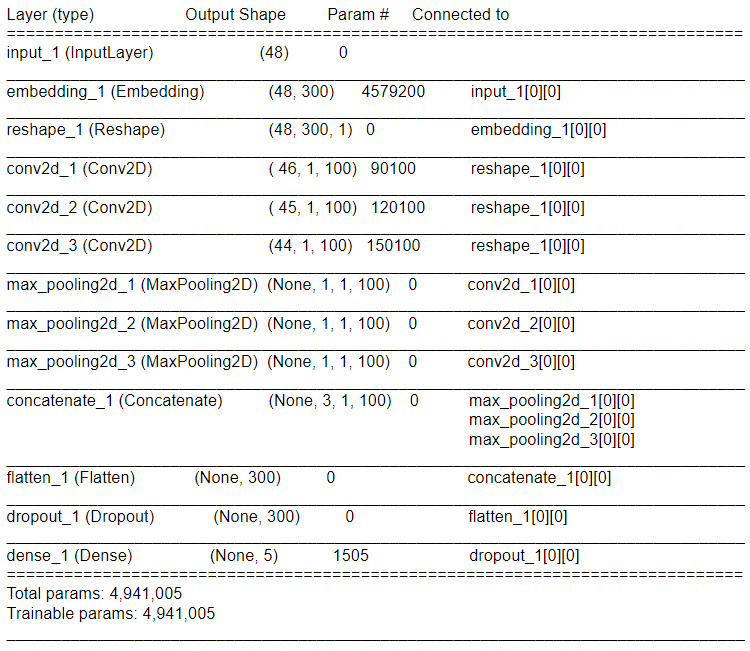
\includegraphics[width=9cm]{summary_cnn.png}
			\label{figure:cnn}
			\ref{figure:cnn}
			\caption{CNN summary}
		\end{figure}
	
	\subsection{LSTM}
	
		Alternatively, LSTM, have require much more data to train and computationally expensive.  Although LSTMs training process is unsupervised/semi-supervised, thus, provides much more flexibility. In particular, Bidirectional LSTM, wich is going to be used, requires twice as much training and computational costs since it incorporates two layers. On the other hand, Bidirectional LSTM produces higher accuracy, since at each step, network has outputs of both layers, front and back sequence at its disposal.
		
		Therefore, it was anticipated, that LSTM should perform better, given a larger dataset, even though it is much less annotated and is lower quality.
		
		First, all trained data is fed to Keras Tokenizer to convert them from words to numeric representation. Next received tokens are provided to Embedding Layer(60x200). After that, Embedding Layer is fed to first Layer of Bidirectional LSTM(60x256). Finally, first Bidirectional LSTM is supplied into other directional Layer of Bidirectional LSTM(128).
		
		Additionally, summary of LSTM can be found at \ref{figure:lstm}, while code for LSTM is available in submition folder, \textbf{\\train\textbackslash train\_LSTM\_RT.py} for \RT and \textbf{\\train\textbackslash train\_LSTM\_TW.py} for \TW.
		
		\begin{figure}
			\centering
			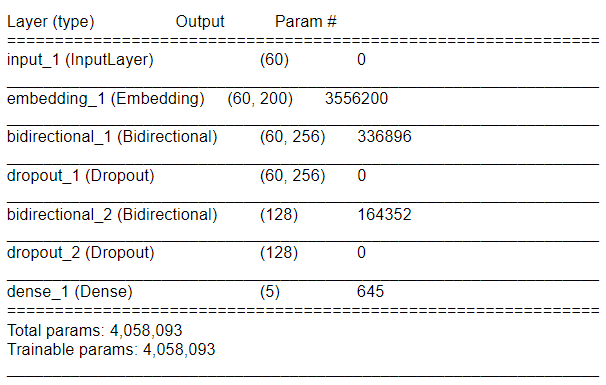
\includegraphics[width=9cm]{summary_lstm.png}
			\label{figure:lstm}
			\ref{figure:lstm}
			\caption{LSTM summary}
		\end{figure}

	\subsection{Dataset}
		While considering two datasets, key factors for selections were the fact that, datasets should be opposite and have clear distinctions. Namely, one of the datasets had to be relatively small, small to medium size, while preserving higher quality of sentiment to train on. Conversely, the other dataset should have been direct oposite of the first, so that, later on it would have been easier to make direct comparison. Thus, \RT\cite{dataset:RT} and \TW\cite{dataset:TW} where selected for those intents.
		
		\subsubsection{\RT\cite{dataset:RT}}
		
			\RT, is a dataset, that consists of movie reviews from RottenTomatoes website. Movie reviews primarily are designed to express the sentiment towards the certain aspects of the movies. 
			
			As it was mentioned, one of the datasets had to be relatively small and should also have higher quality data, thus, \RT\cite{dataset:RT} was considered for the following reasons:

			\begin{enumerate}
				\item \label{itm:RT:1} Small-Medium size(156000x4 size)
				\item \label{itm:RT:2} Dataset preserves higher quality Sentiment 
				\item \label{itm:RT:3} 5 Way Sentiment
			\end{enumerate}
			Cross-referencing items \ref{itm:RT:1} and \ref{itm:RT:2}.
			
			Claim \ref{itm:RT:2} comes from the fact that dataset provides sentiment for each individual element of the sentence. Additionally, example of the sentence from dataset with sentiment for each phrase of the sentence is provided in table \ref{table:1}.
			
			Also, 5 way sentiment encoding is following : 0 - negative, 1 - somewhat negative, 2 - neutral, 3 - somewhat positive, 4 - positive.
			
			
			\begin{table}
				\centering
				\begin{tabular}{ | m{2cm} | m{2cm}| m{5em} | m{2cm} | } 
					\hline
					PhraseID & SentenceID & Sentence & Sentiment \\ %[0.5ex] 
					\hline
					106 & 3 & a hard time sitting through this one & 1 \\ 
					\hline
					107 & 3 & a hard time & 1 \\
					\hline
					108 & 3 & hard time & 1 \\
					\hline
					109 & 3 & hard & 2 \\ [1ex]
					\hline
				\end{tabular}
				\caption{sample from dataset \RT}
				\label{table:1}
				\ref{table:1}
			\end{table}
		
		
		\subsubsection{\TW\cite{dataset:TW}}
			
			\TW\cite{dataset:TW} is a dataset that was collected from twitter, by traversing trough large number of twitter posts. Though, twitter post are considered to have sentiments to certain extent.
			
			Conversely, \TW\cite{dataset:TW}, has direct opposite properties compared to \RT\cite{dataset:RT}. First, as it can be seen from  \ref{table:2}, sentiment is only provided for the hole sentence. Moreover, sentiment is only binary. Second, size of \TW\cite{dataset:TW} dataset is much bigger in contrast with \RT\cite{dataset:RT}, although, much less annotated.
			
		
			\begin{table}
				\centering
				\begin{tabular}{| m{6cm} | m{1cm} | } 
					\hline
					Sentence & Sentiment\\
					\hline
					don't let the sun catch you crying - oh my.. so cool & pos \\ 
					\hline
					the floor just bit my face. & neg \\
					\hline
					definitely smiling & pos \\
					\hline
				\end{tabular}
				\caption{exerpt of dataset \TW}
				\label{table:2}
				\ref{table:2}
			\end{table}

\section{Results}\label{AA}

Categorical Accuracy, Categorical Cross-entropy and Mean Absolute Error(MAE) were used as key metrics for network performance measurements. Also, all of the measurements were obtained while performing tests on different data of the same dataset. For instance, CNN trained on \RT was tested on separate data from same dataset, namely, \RT, that was not used for training 

	\subsection{CNN}
	
		\subsubsection{CNN trained on \RT}
		
			the graph \ref{figure:2} shows, loss function CNN that was trained on \RT, gradually descends reaching 0,7\% by 100 epoch. Meanwhile, Categorical accuracy of  CNN trained on \RT, steadily grows, reaching approximately 0.77\% accuracy by the same time.
			
			\begin{figure}
				\caption{Categorical Crossentropy and MAE. CNN-RT}
				\centering
				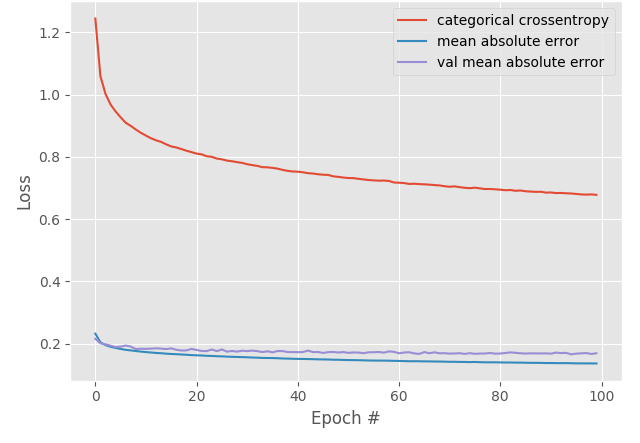
\includegraphics[width=7.5cm]{categorical_crossentropy_mae_cnn-rt.png}
				\label{figure:1}
				\ref{figure:1}
			\end{figure}
			
			\begin{figure}
				\caption{Categorical Accuracy. CNN-RT}
				\centering
				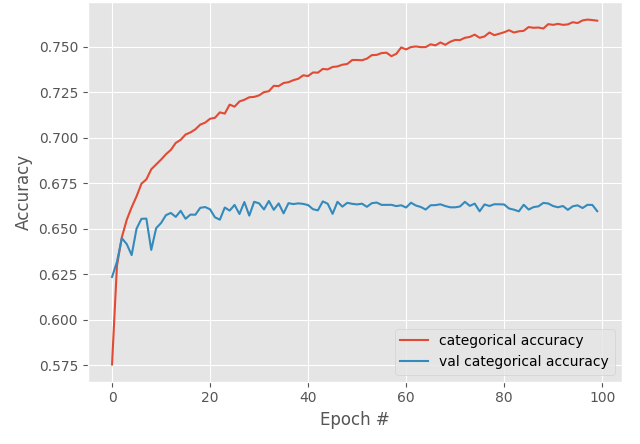
\includegraphics[width=7.5cm]{categorical_accuracy_cnn-rt.png}
				\label{figure:2}
				\ref{figure:2}
			\end{figure}
			
		
		\subsubsection{CNN trained on \TW}
		
			Figures \ref{figure:3} , \ref{figure:4} suggest, that CNN trained on \TW descend from a much higher Categorical Cross-entropy value of about 0.55 and descends much slower up to only 0.38 by 100 epoch, compared to CNN trained on \RT. Though, training accuracy of CNN trained on \TW, is similar to CNN trained on \RT.
			
			\begin{figure}
				\caption{Categorical Crossentropy and MAE. CNN-TW}
				\centering
				\includegraphics[width=7.5cm]{categorical_crossentropy_mae_cnn-TW.png}
				\label{figure:3}
				\ref{figure:3}
			\end{figure}
			
			\begin{figure}
				\caption{Categorical Accuracy. CNN-TW}
				\centering
				\includegraphics[width=7.5cm]{categorical_accuracy_cnn-TW.png}
				\label{figure:4}
				\ref{figure:4}
			\end{figure}
		
		Overall performance of CNN trained using both datasets can be found in table \ref{table:4}
		As it can be seen from the table \ref{table:4}, overall accuracy of CNN trained on \RT, even though, the size of the dataset is relatively small, is much higher, reaching around 0.7934\%, while CNN trained on \TW only produced 0.6406 \%.
		
		while scripts for training CNNs on \RT and \TW can be found at \textbf{\\train\textbackslash train\_CNN\_RT.py}, \textbf{\\train\textbackslash train\_CNN\_TW.py}. Besides, resulting trained model can be found at \cite{report:repo} under \textbf{\textbackslash model}.
		
		\begin{table}
			\centering
			\begin{tabular}{| m{2cm} | m{1.1cm} | m{1.1cm} | m{1.1cm} |  m{1.1cm} | } 
				\hline
				Dataset & Accuracy & Categorical Cross Entropy & Mean Absolute Error & Test Accuracy\\
				\hline
				\RT & 0.845 \% & 0.5512 & 0.1009 & 0.7934 \% \\ 
				\hline
				\TW & 0.879 \% & 0.3845 & 0.2241 & 0.6406 \% \\ 
				\hline
			\end{tabular}
			\caption{summary table for CNN performance}
			\label{table:3}
			\ref{table:3}
		\end{table}
	
	\subsection{LSTM}
	
		\subsubsection{LSTM trained on \RT}
			
			figures \ref{figure:5} and \ref{figure:5} illustrate, that Categorical Cross-entropy constantly declines through the hole period, starting from around 0.80\% at 2 epoch, reaching about 0.18\% by 100 epoch. At the same time, Categorical Accuracy steadily increases from about 0.65\%, and flattening out at about 0.92\% by 100 epoch.
			
			\begin{figure}
				\caption{Categorical Crossentropy and MAE. LSTM-RT}
				\centering
				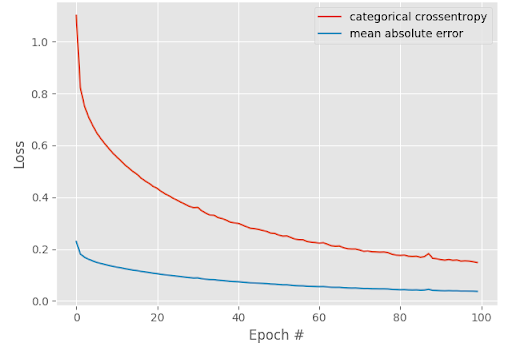
\includegraphics[width=7.5cm]{categorical_crossentropy_mae_lstm-rt.png}
				\label{figure:5}
				\ref{figure:5}
			\end{figure}
			
			\begin{figure}
				\caption{Categorical Accuracy. LSTM-RT}
				\centering
				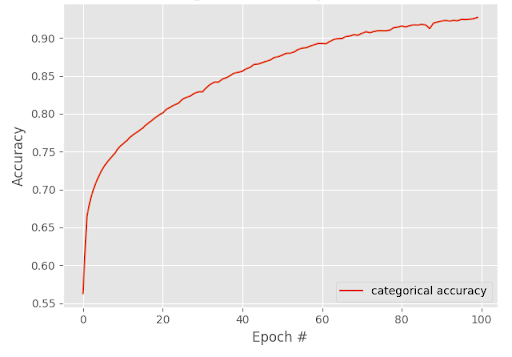
\includegraphics[width=7.5cm]{categorical_accuracy_lstm-rt.png}
				\label{figure:6}
				\ref{figure:6}
			\end{figure}
		
		\subsubsection{LSTM trained on \TW}
		
			Pictures \ref{figure:7} and \ref{figure:8} show that LSTM trained on \RT reached almost 0 Categorical Cross-entropy and MAE and about 0,98\% training accuracy by 100 epoch. That is to suggest, that LSTM trained on \TW over-fitted. Although , the size of the \TW dataset is quite high, it is believed, due to poor quality of the dataset, LSTM was not able to capture sentence structures for further sentiment analysis, thus, resulting in an over-fitted model.
			
			\begin{figure}
				\caption{Categorical Crossentropy and MAE. LSTM-TW}
				\centering
				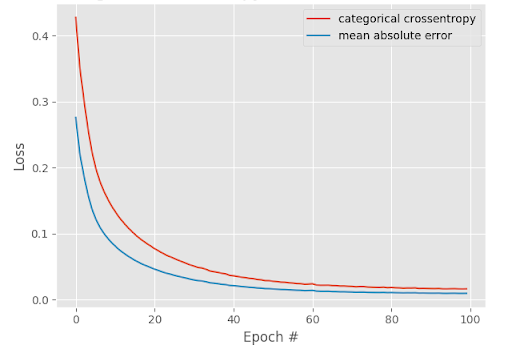
\includegraphics[width=7.5cm]{categorical_crossentropy_mae_lstm-tw.png}
				\label{figure:7}
				\ref{figure:7}
			\end{figure}
			
			\begin{figure}
				\caption{Categorical Accuracy. LSTM-TW}
				\centering
				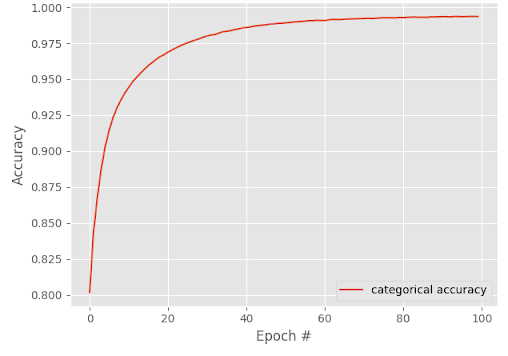
\includegraphics[width=7.5cm]{categorical_accuracy_lstm-tw.png}
				\label{figure:8}
				\ref{figure:8}
			\end{figure}
		
		Summary performance of LSTM trained using both datasets can be found in table \ref{table:4}
		Numbers that can be found in table \ref{table:4} suggest, that, LSTM trained on \RT produces tremendous results reaching nearly 0.94 \% accuracy on tests. On the other hand, LSTM trained on \TW over-fitted, therefore, producing low test accuracy, that is only 54\% 
		
		Similarly to CNN scripts for LSTMs training on \RT and \TW can be found at \textbf{\\train\textbackslash train\_LSTM\_RT.py}, \textbf{\\train\textbackslash train\_LSTM\_TW.py}. Besides, resulting trained model can be found at \cite{report:repo} under \textbf{\textbackslash model}.
		
		\begin{table}
			\centering
			\begin{tabular}{| m{2cm} | m{1.1cm} | m{1.1cm} | m{1.1cm} |  m{1.1cm} | } 
				\hline
				Dataset & Accuracy & Categorical Cross Entropy & Mean Absolute Error & Test Accuracy\\
				\hline
				\RT & 0.945 \% & 0.1464 & 0.0842 & 0.9389 \% \\ 
				\hline
				\TW & 0.989 \% & 0.0025 & 0.0012 & 0.5419 \% \\ 
				\hline
			\end{tabular}
			\caption{summary table for CNN performance}
			\label{table:4}
			\ref{table:4}
		\end{table}
		
	\subsection{Demo}
		Finally, to illustrate the final results fo trained models, small demo scripts were written up so that they can predict sentiment for a give sentences. Moreover, sources for demo scripts are located in \textbf{demo\_CNN\_RT.py}, \textbf{demo\_CNN\_TW.py}, \textbf{demo\_LSTM\_RT.py}, \textbf{demo\_LSTM\_TW.py},

\section{Conclusion}

\begin{table}
	\centering
	\begin{tabular}{| m{1.1cm} | m{2cm} | m{1.1cm} | m{1.1cm} | m{1.1cm} |  m{1.1cm} | } 
		\hline
		Model & Dataset & Accuracy & Categorical Cross Entropy & Mean Absolute Error & Test Accuracy\\
		\hline
		CNN & \RT & 0.845 \% & 0.5512 & 0.1009 & 0.7934 \% \\ 
		\hline
		CNN & \TW & 0.879 \% & 0.3845 & 0.2241 & 0.6406 \% \\ 
		\hline
		LSTM & \RT & 0.945 \% & 0.1464 & 0.0842 & 0.9389 \% \\ 
		\hline
		LSTM & \TW & 0.989 \% & 0.0025 & 0.0012 & 0.5419 \% \\ 
		\hline
	\end{tabular}
	\caption{Summary Table}
	\label{table:5}
	\ref{table:5}
\end{table}

To conclude, as it can be seen from table \ref{table:5}, dataset had a higher impact on overall accuracy than the sophistication of the method, although additional complexity allowed further development of the area, enabling Aspect Level Sentiment Analysis.


%\section*{Acknowledgment}
%
%The preferred spelling of the word ``acknowledgment'' in America is without 
%an ``e'' after the ``g''. Avoid the stilted expression ``one of us (R. B. 
%G.) thanks $\ldots$''. Instead, try ``R. B. G. thanks$\ldots$''. Put sponsor 
%acknowledgments in the unnumbered footnote on the first page.

%\vspace{12pt}

\clearpage
\footnotesize{
	%\bibliographystyle{plainnat}
	%\bibliographystyle{ieeetr}
	\bibliography{ref}
}

\end{document}
